%----------------------------------------------------------------%
%--------------------------INFORMATIONEN-------------------------%
%----------------------------------------------------------------%
%	Infos gibt es zu jedem Paket auf www.ctan.org
%	Werden bei den Paketen bestimmte Optionen gesetzt, so sind die Wichtigsten erklaert
%	solange sie nicht selbsterklärend sind

%----------------------------------------------------------------%
%--------------------------GRUNDEINSTELLUNGEN--------------------%
%----------------------------------------------------------------%
\documentclass[11pt, oneside, ngerman, footinclude=off, captions=tableheading, DIV=12, headerinclude=false, headings=optiontohead]{scrartcl}
\usepackage[bottom=2.5cm, inner=2.5cm, outer=2.5cm, top=2.5cm]{geometry}
%	'oneside'/'twoside': nicht zwischen linker und rechter Seite unterscheiden (alternativ twoside)
%	'twocolumn': wuerde 2 Spalten auf dem Blatt platzieren
%	'bibliography=totocnumbered': Normal nummeriertes Inhaltsverzeichnis (Kapitelnummer)
%	'listof=totocnumbered': Abbildungs- und Tabellenverzeichnis normal nummeriert (Kapitelnummer)
%	'ngerman' verwendet deutsch als Dokumentensprache (z.B. fuer Sirange)
%	'footinclude=off': Zaehlt Fusszeile zum Rand (vergroessert den Textbereich)
%	'captions=tableheading': Tabellenueberschriften explizit verwenden, erhoeht den Abstand zur Tabelle
%	'DIV=12': Kleinere Seitenraender (s. hierzu die KOMA-Documentation)

\usepackage[ngerman, english]{babel}							%	Einstellen der Sprache
\usepackage[T1]{fontenc}							%	Wie wird Text ausgegeben, d.h. im PDF
\usepackage[utf8]{inputenc}							%	Welche Zeichen 'versteht' LaTeX bei der Eingabe?
%\usepackage{lmodern}								%	Laedt Schriften, die geglaettet sind
\usepackage{helvet}     % Helvetica laden (Arial-Ersatz)
\renewcommand{\familydefault}{\sfdefault} % S			
			
											
\usepackage{blindtext}								%	Beispieltext, zum Testen geeignet
%\usepackage{showframe}
%----------------------------------------------------------------%
%--------------------------ABSTÄNDE------------------------------%
%----------------------------------------------------------------%
\usepackage[singlespacing]{setspace}				%	Für Zeilenabstaende: 'singlespacing' (einfach), 'onehalfspacing' (1.5-fach), 'doublespacing' (2fach)
%\setlength{\parindent}{0cm}						%	Laengenangabe für die Einrueckung der ersten Zeile eines neuen Absatzes.
%\setlength{\parskip}{6pt plus 3pt minus 3pt}		%	Laengenangabe für den Abstand zwischen zwei Absaetzen.
%	Wenn diese beiden Befehle nicht kommentiert sind, wird ein Absatz nicht eingezogen sondern es gibt einen Abstand

%----------------------------------------------------------------%
%--------------------------MATHE---------------------------------%
%----------------------------------------------------------------%
\usepackage[]{mathtools}							%	Erweiterung von AMSMath, laedt automatisch AMSMath - für viele Mathe-Werkzeuge, 'fleqn' als Option ist für Mathe linksbuendig
\usepackage{amsfonts}								%	Für eine Vielzahl an mathematischen Symbolen

%----------------------------------------------------------------%
%--------------------------KOPF- UND FUSSZEILEN------------------%
%----------------------------------------------------------------%
\usepackage[automark,headsepline=.4pt]{scrlayer-scrpage}
\pagestyle{scrheadings}
\setkomafont{pageheadfoot}{\normalfont\bfseries}	%	Normale Schriftart und Fett für den Seitenkopf
\addtokomafont{pagenumber}{\normalfont\bfseries}	%	Normale Schriftart und Fett für die Seitenzahl

\clearscrheadfoot
\ohead{\thepage}									%	Rechter Seitenkopf mit Seitenzahl
\ihead{\headmark}									%	Linker Seitenkopf mit section
\ofoot[]{\empty}
%\ofoot{\thepage}									%	Leere Fußzeile, ungerade Seiten
%	Definert man oben in der documentclass 'twoside', so wird zwischen geraden und ungeraden Seiten unterschieden (NUR DANN!)

%----------------------------------------------------------------%
%--------------------------BILDER--------------------------------%
%----------------------------------------------------------------%
\usepackage{graphicx}									%	Um Bilder einbinden zu koennen 
\usepackage[dvipsnames,svgnames,table]{xcolor}			%	Farben verwenden, Versch. Farbdefinitionen, Farben in Tabellen (-Reihen, -Spalten)
\usepackage{pdfpages}									%	pdfs importieren
\definecolor{Seeblau100}{RGB}{0,169,224}				%	Uni-Farben, z.B. fuer Tabellen
\definecolor{Seeblau65}{RGB}{89,199,254}
\definecolor{Seeblau35}{RGB}{165,224,254}
\definecolor{Seeblau20}{RGB}{203,237,254}
\definecolor{Seegrau60}{RGB}{102,102,102}
\definecolor{Seegrau40}{RGB}{153,153,153}
\definecolor{Seegrau20}{RGB}{204,204,204}
\definecolor{Seegrau10}{RGB}{230,230,230}

%----------------------------------------------------------------%
%--------------------------POSITIONIERUNG------------------------%
%----------------------------------------------------------------%
\usepackage{float}

%----------------------------------------------------------------%
%--------------------------LISTEN--------------------------------%
%----------------------------------------------------------------%
\usepackage{enumitem}							%	Um Listen / Aufzaehlungen leichter zu modifizieren
%\setlist{noitemsep}							%	Verringert den Abstand in Aufzaehlungen

%----------------------------------------------------------------%
%--------TABELLEN-/BILDUNTERSCHRIFTEN und NUMMERIERUNG-----------%
%----------------------------------------------------------------%
\addtokomafont{captionlabel}{\bfseries}			%	Abbildung X.Y wir fett geschrieben
\setcapindent{2em}								%	2. Zeile teilweise haengend und eingezogen. Wenn ganz haengend gewuenscht, auskommentieren

\numberwithin{equation}{section}				%	Nummerierung der Gleichungen, Tabellen und Bilder nach der Kapitelnummer
\numberwithin{figure}{section}
\numberwithin{table}{section}

%----------------------------------------------------------------%
%--------------------------LITERATURVERZEICHNIS------------------%
%----------------------------------------------------------------%
\usepackage[german]{babelbib}					%	Bereitstellung des deutschen Layouts fuer die Bibliography

%----------------------------------------------------------------%
%--------------------------SIUNITX-------------------------------%
%----------------------------------------------------------------%
\usepackage[]{siunitx}
\sisetup{locale = DE}							%	Automatische Einstellung der Ausgabe für bestimmte Regionen (UK, US, DE, FR, ZA)

%----------------------------------------------------------------%
%--------------------------URLs / REFs---------------------------%
%----------------------------------------------------------------%
\usepackage[hidelinks]{hyperref}				%	Erweiterte Referenzierung ('hidelinks' verhindert Linien um Links)

%----------------------------------------------------------------%
%--------------------------EIGENE BEFEHLE------------------------%
%----------------------------------------------------------------%
\usepackage{mhchem}
%\usepackage{subfig}
\usepackage{subcaption}
\usepackage{listings}
%\lstset{numbers=none}
\definecolor{backcolour}{rgb}{0.95,0.95,0.92}
%\lstset{
%	numbers=none,
%	language=HTML,
%	breaklines=true,
%	frame=single,
%	tabsize=2,
	%backgroundcolor=\color{backcolour},  
%}

%\lstset{
%  language=HTML,
%  basicstyle=\ttfamily\small,
%  keywordstyle=\color{blue},
%  stringstyle=\color{red},
%  commentstyle=\color{green!50!black},
%  showstringspaces=false,
%  breaklines=true,
%  frame=single
%}

\definecolor{lightgray}{rgb}{.9,.9,.9}
\definecolor{darkgray}{rgb}{.4,.4,.4}
\definecolor{purple}{rgb}{0.65, 0.12, 0.82}

\lstdefinelanguage{JavaScript}{
  keywords={typeof, new, true, false, catch, function, return, null, catch, switch, var, if, in, while, do, else, case, break},
  keywordstyle=\color{blue}\bfseries,
  ndkeywords={class, export, boolean, throw, implements, import, this},
  ndkeywordstyle=\color{darkgray}\bfseries,
  identifierstyle=\color{black},
  sensitive=false,
  comment=[l]{//},
  morecomment=[s]{/*}{*/},
  commentstyle=\color{purple}\ttfamily,
  stringstyle=\color{red}\ttfamily,
  morestring=[b]',
  morestring=[b]"
}

\lstset{
   language=JavaScript,
   backgroundcolor=\color{lightgray},
   extendedchars=true,
   basicstyle=\footnotesize\ttfamily,
   showstringspaces=false,
   showspaces=false,
   numbers=left,
   numberstyle=\footnotesize,
   numbersep=9pt,
   tabsize=2,
   breaklines=true,
   showtabs=false,
   captionpos=b
}


\usepackage{makecell}


\begin{document}
	%---------------------------------------------------------------------------------------------%
	%------------------------------------------TITELSEITE-----------------------------------------%
	%---------------------------------------------------------------------------------------------%
	\title{Project}
	\subtitle{AI in Transportation}
	\author{Author: Johanna Schaefer}
	\date{17.10.2025}
	\maketitle
	\vspace{3cm}
	\pagenumbering{alph}	% Griechische (unsichtbare) Seitenzahlen, damit kein doppeltes Vorkommen
	
	\thispagestyle{empty}	% Seite ohne Seitenkopf
	
	
	%\newpage 
	\thispagestyle{empty}
	
	
	
	\thispagestyle{empty}
	\cleardoublepage
	\thispagestyle{empty}
	\newpage
	
	%---------------------------------------------------------------------------------------------%
	%------------------------------------------INHALTSVERZEICHNIS---------------------------------%
	%---------------------------------------------------------------------------------------------%
	%\tableofcontents
	%\thispagestyle{empty}	% Seite ohne Seitenkopf
	%\newpage
	\setcounter{page}{1}	% Seitenzahle auf 1 Setzen
	\pagenumbering{arabic}	% Arabische Seitenzahlen
	
	%---------------------------------------------------------------------------------------------%
	%------------------------------------------DOKUMENTENKÖRPER-----------------------------------%
	%---------------------------------------------------------------------------------------------%
	\section{Introduction}
	In modern transport systems, continuous collection of traffic data is essential for providing real-time information on speed and traffic flow. Sensors on road portals provide important data, but if individual sensors fail or provide incomplete data, this can affect the accuracy of predictions. The central question of this work is therefore: How well can missing sensors be compensated for by data from other sensors in the same portal or from neighbouring portals?
	To answer this question, a regression approach is used in which the measured values of a target sensor are predicted on the basis of neighbouring sensors. The study examines whether sensors within the same portal provide better prediction accuracy than sensors from a neighbouring portal. 
	%The aim is to analyse the spatial and temporal relationships between sensors, identify factors influencing prediction performance, and thus gain insights for more robust traffic data collection.
	%The work combines descriptive analysis, feature engineering, and various machine learning methods, including linear models, XGBoost, and neural networks, to develop a deeper understanding of data relationships and prediction potential.
	
	\section{Descriptive analysis}
	To begin the project of creating predictive models of the data provided, the data needs to be analysed.
	
	\subsection{Data description}
	The data set used for this project consists of speed and traffic flow data from several sensors on the motorway near Stockholm. The data comes from 29 sensors belonging to 8 different portals on a section heading south. Every sensor measures the speed and flow in one line of the motorway. There are inflows and outflows within this section between the portals as can be seen in figure \ref{fig:overview}.
	\begin{figure}[H]
		\centering
		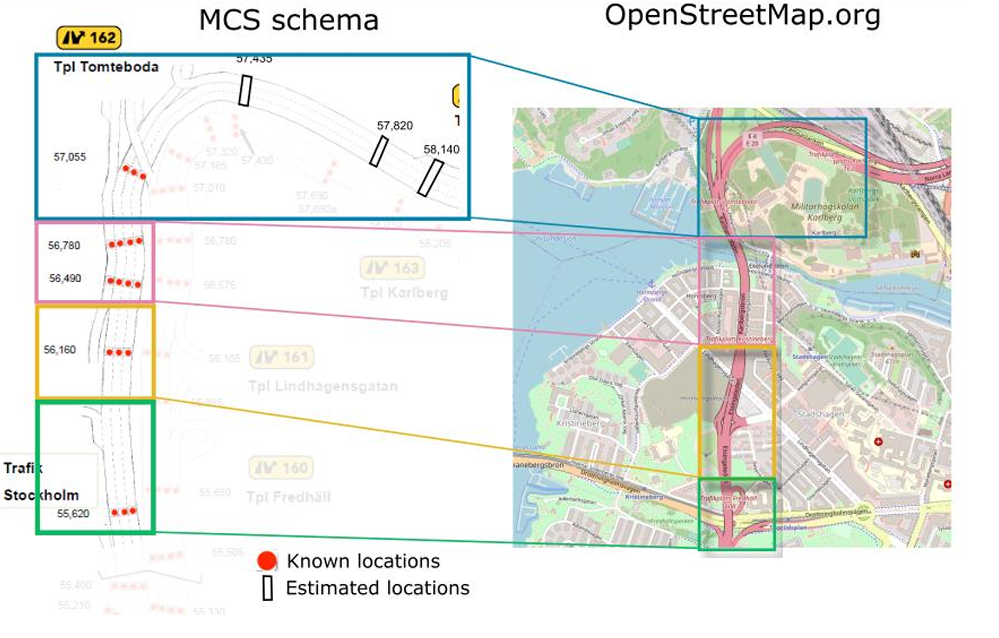
\includegraphics[width=0.7\linewidth]{screenshots/overview}
		\caption{Overview motorway section and portals}
		\label{fig:overview}
	\end{figure}
	\noindent Table \ref{tab:portalsandsensors} shows the portals and the correspondings sensors.
	\begin{table}[H]
		\centering
		\caption{Portals and sensors}
		\label{tab:portalsandsensors}
		\begin{tabular}{|l|l|}
			\hline
			Portal & sensors \\
			\hline
			E4S 55620 & 751, 1254, 1076 \\
			E4S 56160 & 539, 536, 740 \\
			E4S 56490 & 351, 4873, 153, 902 \\
			E4S 56780 & 543, 534, 4872, 1079 \\
			E4S 57055 & 353, 1443, 749 \\
			E4S 57435 & 4430, 4429, 4437 \\
			E4S 57820 & 4427, 4436, 4428, 4439 \\
			E4S 58140 & 4494, 4473, 4495, 4472, 4496 \\
			\hline
		\end{tabular}
	\end{table}
	Over a total of 214 days, speed and flow data were recorder between 4 AM and 10 AM with a temporal resolution of one minute.
	Speed is measured in $\si{m/s}$, while flow is quantified as the number of vehicles per minute.
	\subsection{Speed and Flow over the morning peak}
	Between 9 AM and 10 AM, the flow of vehicles shows a generally increasing trend, indicating a continued buildup of traffic volume as the morning progresses. The rate at which it in increasing is slowing down when approaching the 10 AM. In contrast, the average speed tends to decline over the same period, reflecting growing congestion.
	This inverse relationship between flow and speed is characteristic of peak-hour dynamics, where higher vehicle density leads to reduced travel speeds.
	
	\begin{figure}[H]
		\centering
		\begin{subfigure}{0.7 \linewidth}
			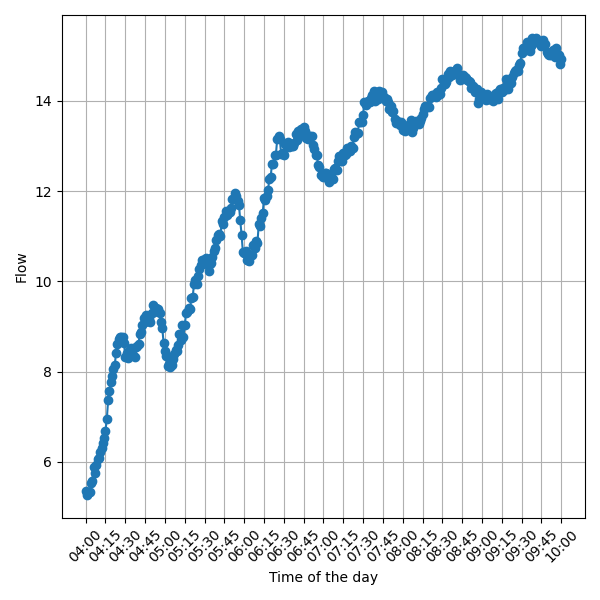
\includegraphics[width=\textwidth]{../Plots/Flow/avg_flow_day}
			\caption{Flow}
		\end{subfigure}
		\begin{subfigure}{0.7 \linewidth}
			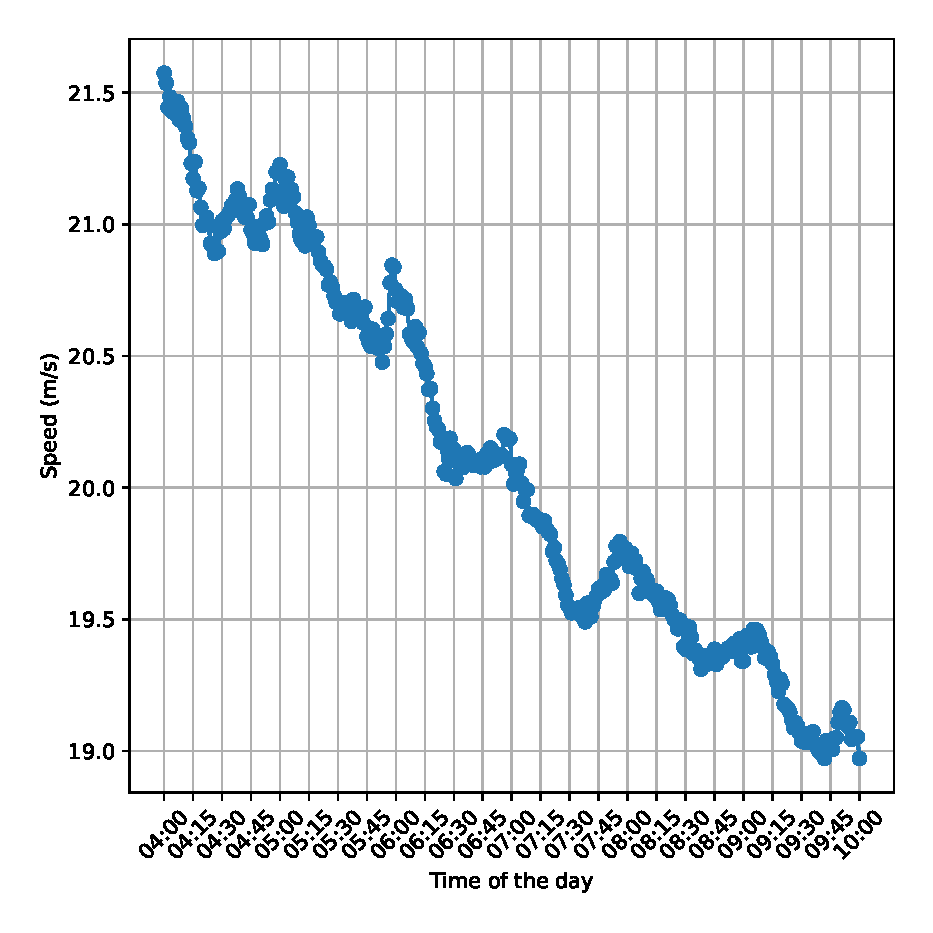
\includegraphics[width=\textwidth]{../Plots/Speed/avg_speed_day}
			\caption{Speed}
		\end{subfigure}
		\caption{Flow and Speed over the day}
	\end{figure}
	\subsection{Correlation}
	Furthermore, the correlation between different sensors was analysed for both speed and flow. It is important to note that no time lag was considered in this initial assessment. In addition to variations in speed and flow across sensors, spatial separation plays a significant role: the greater the distance between sensors, the more pronounced the temporal offset and divergence in observed traffic patterns. In figure \ref{fig:sensor_corr_by_portal} the sensors are displayed grouped by the portals they are part of. The thicker black lines indicate the portals.
	\begin{figure}[H]
		\centering
		\begin{subfigure}{0.9 \linewidth}
			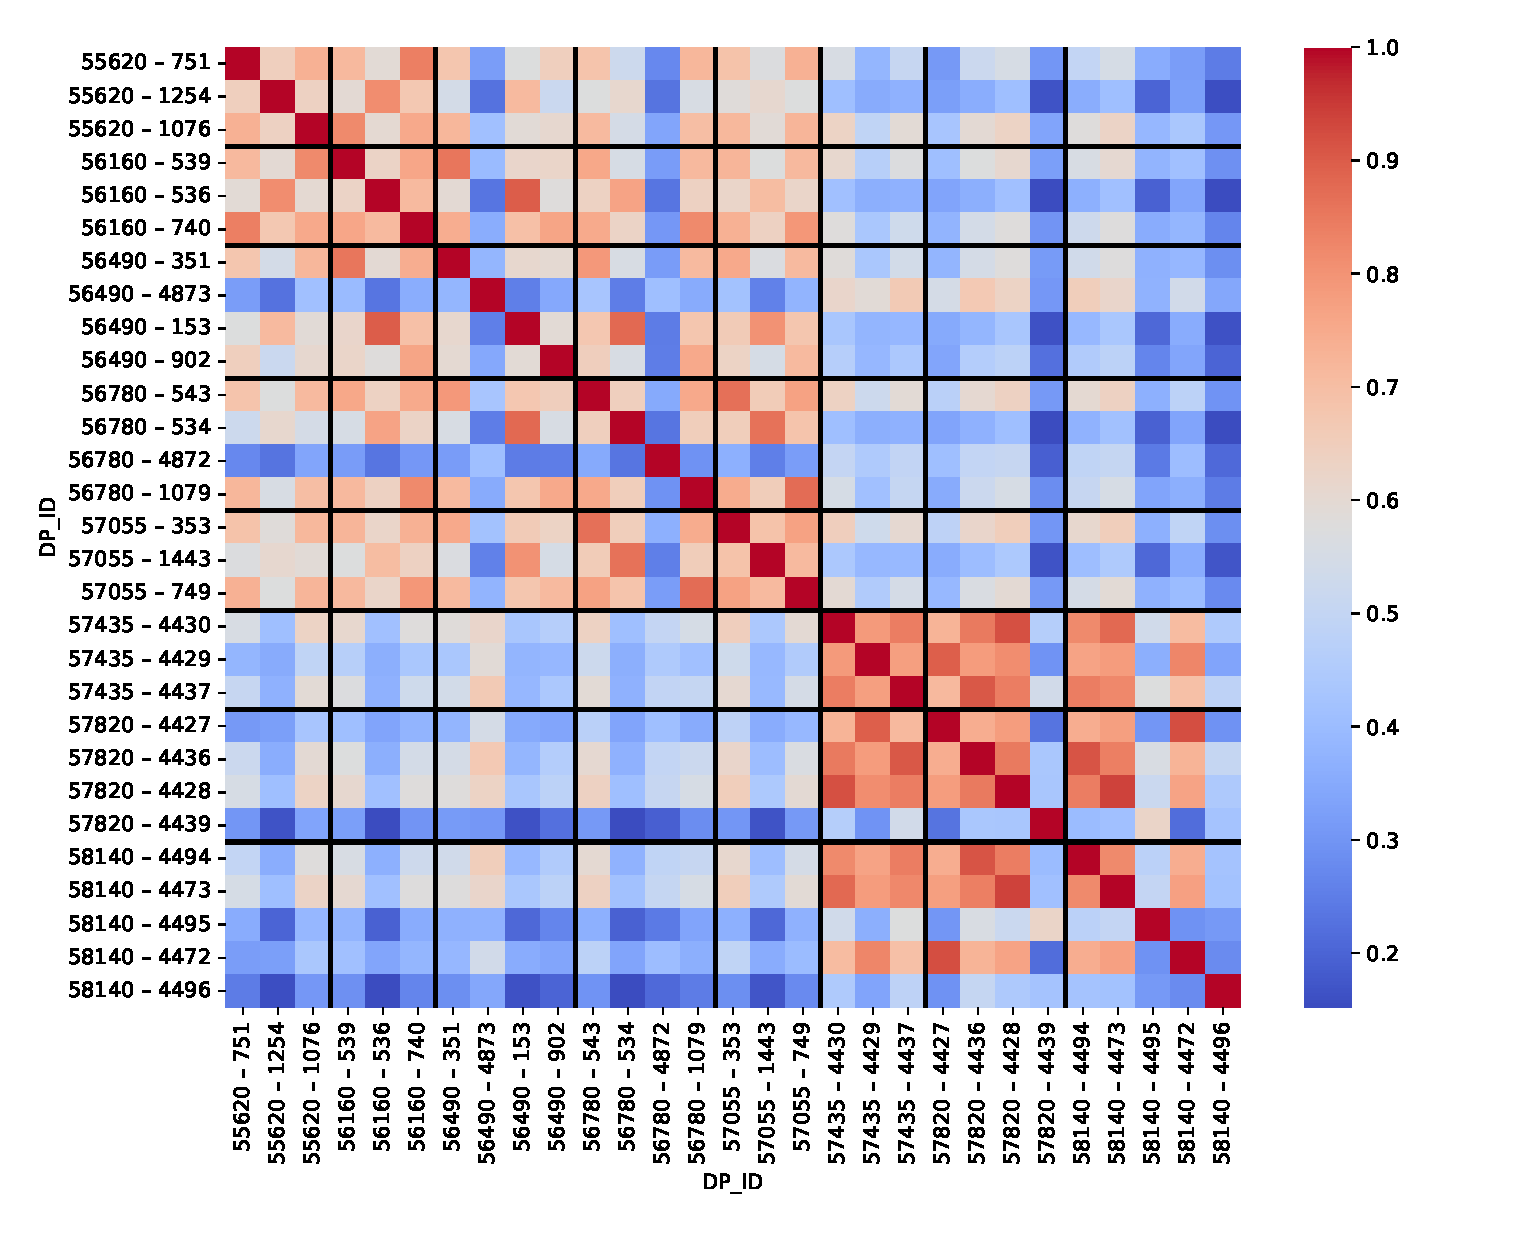
\includegraphics[width=\textwidth]{../Plots/Flow/sensor_corr_by_portal}
			\caption{Flow}
		\end{subfigure}
		\begin{subfigure}{0.9 \linewidth}
			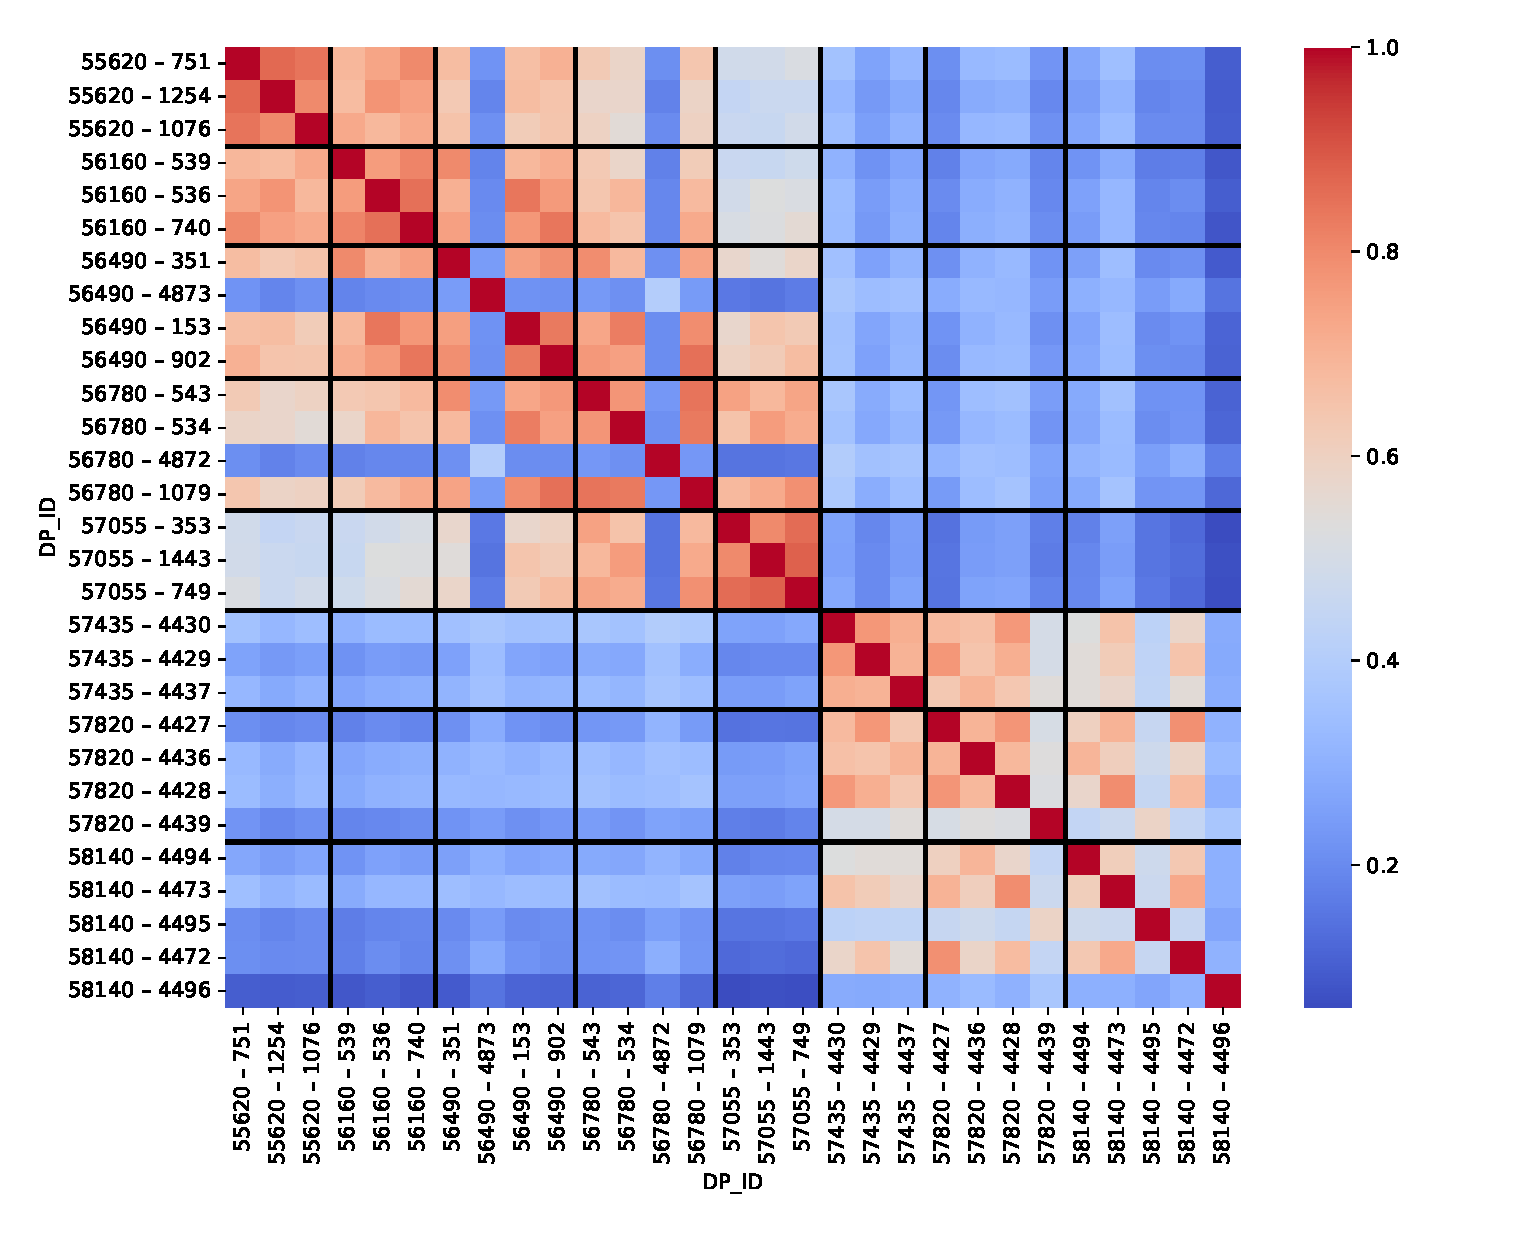
\includegraphics[width=\textwidth]{../Plots/Speed/sensor_corr_by_portal}
			\caption{Speed}
		\end{subfigure}
		\caption{Correlation between speed and flow in different sensors}
		\label{fig:sensor_corr_by_portal}
	\end{figure}
	\noindent Two very interesting finding can be found from this correlation matrix. First of all, it can be seen that it seems like there are two different groups of portals. Portal 55620, 56160, 56490, 56780 and 57055 are more similar to each other than to the other three, that also seem to form a group. 
	Furthermore, speed and flow show different patterns. It can be seen that for the speed the correlation is generally higher within the same portal (indicated by high density of red squares close to the diagonal). On the other side, this is not necessarily the case for the flow values. It can be seen that the red squares are more spread out, showing that the correlation is also partially quite high with sensor data from other portals.
	\subsection{Clustering as lane identification}
	As part of the data analysis, lane identification was performed using unsupervised clustering.
	The underlying assumption is that different lanes exhibit distinct traffic characteristics in terms of speed and flow. Typically, faster lanes are located on the left (e.g., overtaking lanes), while slower lanes are positioned on the right (e.g., exit or merging lanes). It was hoped to find these behaviour patterns in the sensor data to infer lane structure.
	To uncover these latent lane groupings, K-Means clustering was used. It was chosen among several other clustering methods as it is the easiest method to control the number of clusters which should in the best case- represent the lanes.
	Based on the pattern that was observed in the correlation matrix showing two different portals groups, they were clustered separately. 
	For the five portals, the number of clusters was set to 4 according to the number of lanes.
	Figure \ref{fig:clustering_5portals} shows the typical dayprofil for the different clusters that were identified.
	\begin{figure}[H]
		\centering
		\begin{subfigure}{0.9 \linewidth}
			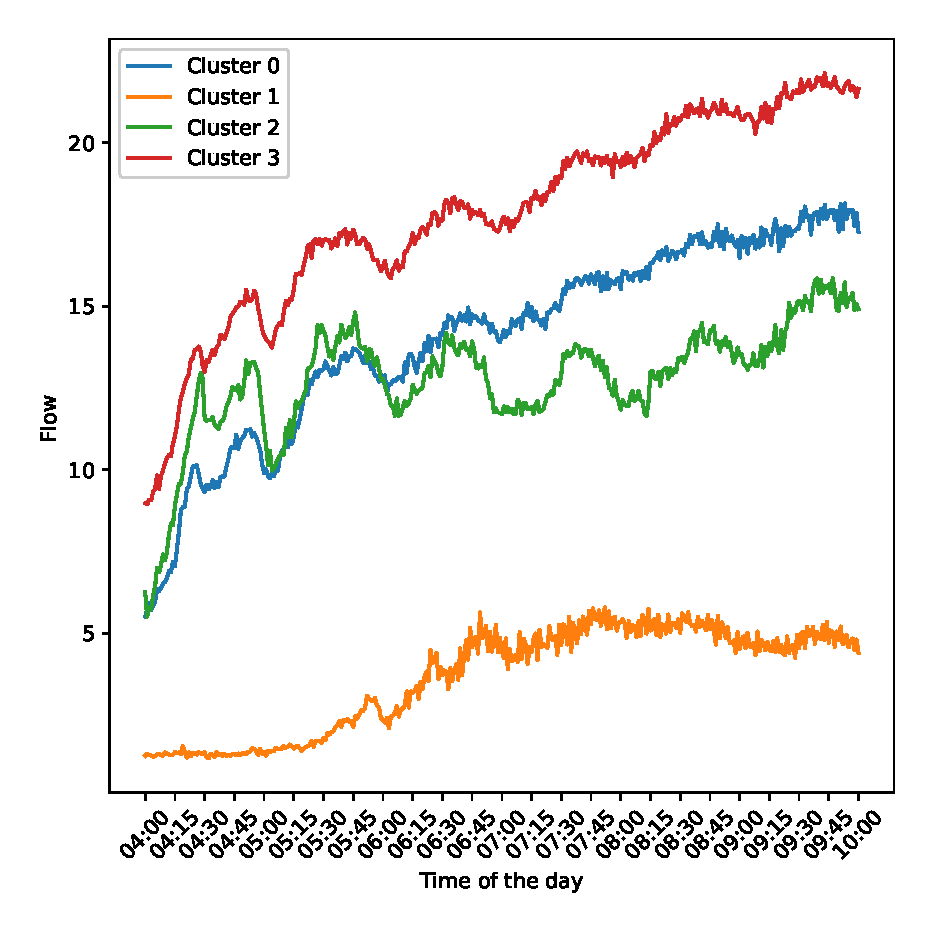
\includegraphics[width=\textwidth]{../Plots/Flow/clustering_5portals}
			\caption{Flow}
		\end{subfigure}
		\begin{subfigure}{0.9 \linewidth}
			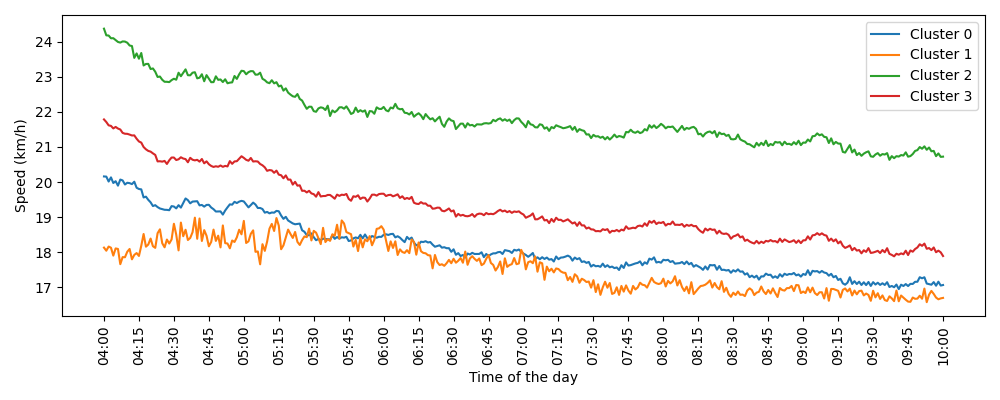
\includegraphics[width=\textwidth]{../Plots/Speed/clustering_5portals}
			\caption{Speed}
		\end{subfigure}
		\caption{blabla}
		\label{fig:clustering_5portals}
	\end{figure}
	Based on these patterns it is very likely -though not proven - that cluster 2 corresponds to the leftest lane showing the highest speed, cluster 3 corresponds to the middle lane with a lower speed, cluster 0 the the right lane and cluster 1 to the lane where cars enter and leave the motorway with the lowest flow.
	
	
	\subsection{Data preprocessing}
	\subsection{Further descriptive analysis for the portal 55620 and 56160}
	\subsubsection{Correlation with lag-data}
	Furthermore, 
	The speed graph shows a clear transition from a steep to a flat correlation curve at lag $\approx  15$, with a secondary drop at lag $\approx 25$.
	For FLOW, on the other hand, no clear break is apparent.
	A fixed threshold of lag = 15 was chosen to capture the relevant time delays to.
	\begin{figure}[H]
		\centering
		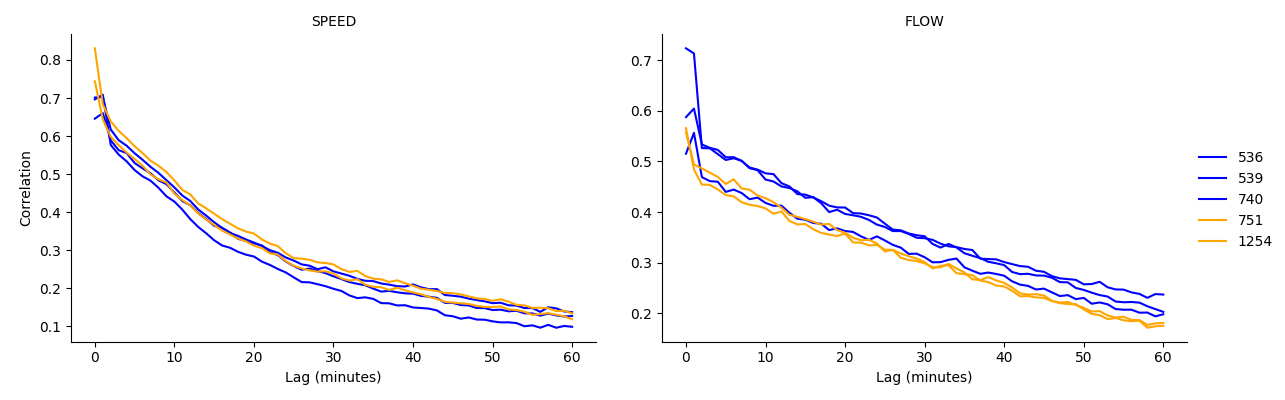
\includegraphics[width =0.99 \linewidth]{../Plots/Correlation_lag_flow_speed_peak}
		\caption{blabla}
		\label{fig:correlation_lag}
	\end{figure}

	\subsubsection{title}
	\section{Problem formulation}
	
	Formulate your speed or flow prediction problem and justify it by discussing its reasonableness for practical use in real-time application. For example,   
	
	What to predict? – Do you predict flow, speeds, or both?
	What is the problem type? – Formulate as a clustering problem, a regression problem, a classification problem, or a combination of these? 
	What features to use? - Develop a-priori hypotheses about features you think are important in predicting 15, 30, 60 minutes in the future. 
	
	\section{Methodology and evaluation methods}
	
	
	\section{Model development}
	
	Data Preprocessing: Clean and preprocess the dataset if necessary, data normalization, and converting categorical variables into suitable formats for modeling.
	Feature Engineering: Analyze the dataset to identify relevant features that could impact bus arrival times. Create new features if necessary, such as time-based features, distance-related features, and aggregation of historical data.
	Exploratory Data Analysis (EDA): Perform EDA to gain insights into the relationships between different variables and bus arrival times. Visualize patterns, correlations, and outliers in the data.
	Model Selection: Select appropriate machine learning algorithms for short-term prediction task. Consider conventional machine learning models or deep neural network models depending on the nature of the data. 
	Model Training: Split the dataset into training and validation sets. Train the selected models using the training data and fine-tune hyperparameters to achieve optimal performance.
	Model Evaluation: Evaluate the trained models using appropriate evaluation metrics such as Mean Absolute Error (MAE), Root Mean Squared Error (RMSE), and Mean Absolute Percentage Error (MAPE). Compare the performance of different models to select the best-performing one. For a comparative analysis, you need to develop at least three different types of models. 
	\section{Model diagnostics}
	
	Design different scenarios to explore how the best model works overall. When and where it does not work? Is it robust to noisy and missing data in real-time? Is it generalizable over months?  
	
	\section{Model deployment}  
	
	
	
	
	\section{Summary of main findings and future works}
	
	
	\appendix
	
	\section{GitHub code link}
	The project can be accessed under:
	\url{https://github.com/Jojo18-20/Project_AI_Transportation}
	
	\section{Additional graphs}
	\begin{figure}[H]
		\centering
		\begin{subfigure}{0.9 \linewidth}
			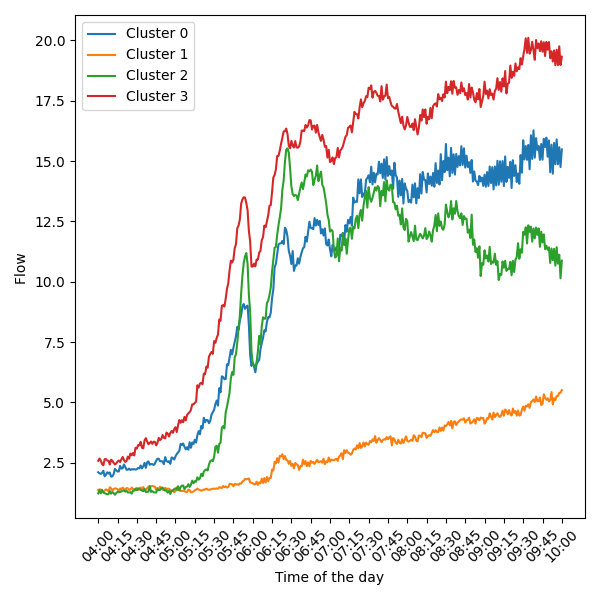
\includegraphics[width=\textwidth]{../Plots/Flow/clustering_3portals}
			\caption{Flow}
		\end{subfigure}
		\begin{subfigure}{0.9 \linewidth}
			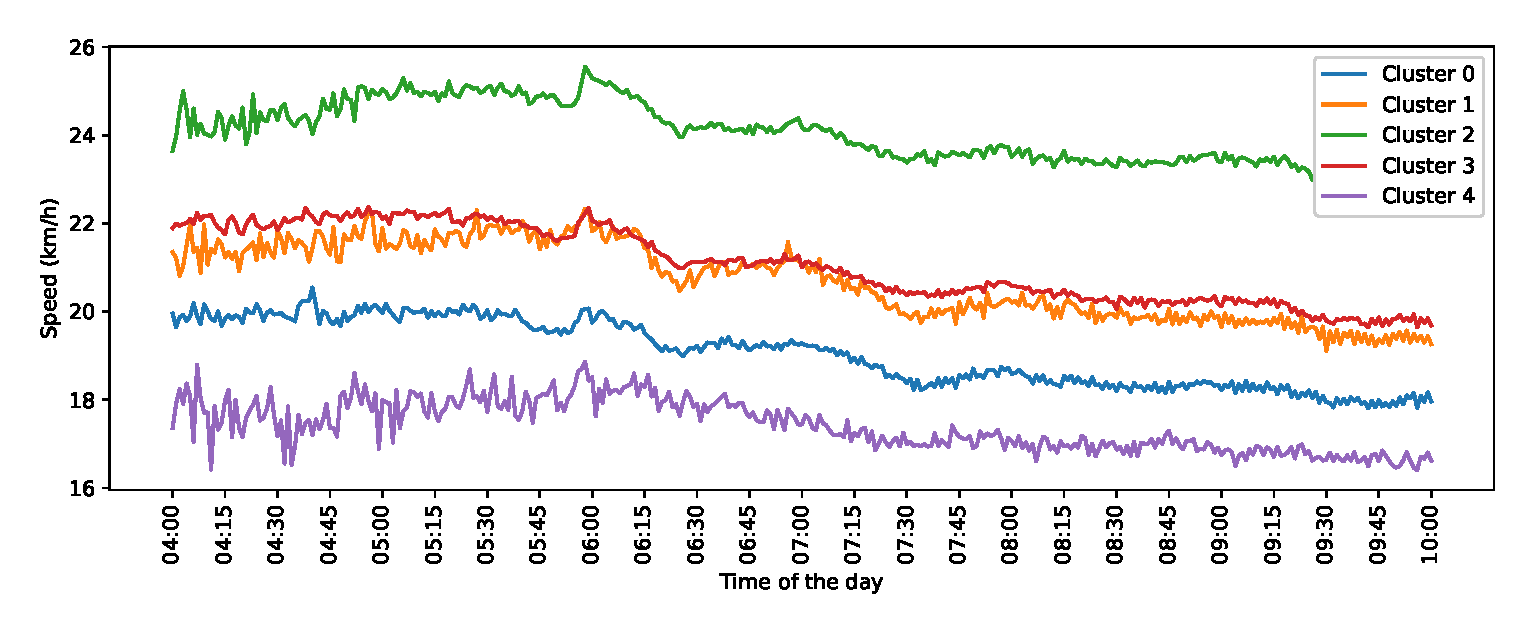
\includegraphics[width=\textwidth]{../Plots/Speed/clustering_3portals}
			\caption{Speed}
		\end{subfigure}
		\caption{Clustering of the three other portals, the exact location of these sensors is not known, thus no interpretation is made on the cluster-lane }
		\label{fig:clustering_3portals}
	\end{figure}
	-------------------------------------------------------------------------%
	%------------------------------------------QUELLENVERZEICHNIS---------------------------------%
	%---------------------------------------------------------------------------------------------%
	%\newpage 
	
	\newpage
	%\bibliography{literatur}
	%\bibliographystyle{babalpha}
	%\bibliographystyle{unsrt}
	%\bibliographystyle{IEEEtran}
	
	%---------------------------------------------------------------------------------------------%
	%------------------------------------------ABBILDUNGSVERZEICHNIS------------------------------%
	%---------------------------------------------------------------------------------------------%
	%\listoffigures
	
	%---------------------------------------------------------------------------------------------%
	%------------------------------------------TABELLENVERZEICHNIS--------------------------------%
	%---------------------------------------------------------------------------------------------%
	%\listoftables
	
	%---------------------------------------------------------------------------------------------%
	%------------------------------------------ANHÄNGE--------------------------------------------%
	%---------------------------------------------------------------------------------------------%
	% Hier kann noch das Messprotokoll als eingescannte PDF angehängt werden 
	%\includepdf{dateiname}
	
	
\end{document}
